
\section{信号検出}

精密な測距・時刻同期のためには精密な信号検出が必要である.
信号検出の誤差は
スマートデバイスのサンプリング周波数は44100Hz
として
1サンプルあたりの時間解像度は約 1/44100 = 22.6μs
であるので,
1サンプルあたりの距離解像度は 22.6μs*340m/s=7.7mm(音速340m/sと仮定)
である.

人間の聴覚特性として,第一波面の法則という現象が知られている\cite{Haas}.
これは二つの音源からの音声が互いに50ms以上ずれると別の音源として知覚されるというものである.

この場合許容される誤差は
$\pm$ 50msの誤差におよそ $\pm$ 2205サンプル以内とかなり緩いものになる.
しかしながらこれでは距離誤差が $\pm$ 3.4m ととても大きなものになってしまう.
というわけで許容される誤差は音像定位よりもむしろ距離測定の手法によって定められる.
今回のような室内空間であれば,
$\pm$ 50cmの誤差つまり $\pm$ 64サンプル以内でパルスを同定できればよいとする.

そこで,そのような高精度のパルス検出をするため,
直接スペクトル拡散方式によるパルス圧縮で高いSN比を向上させ,
信号検出には通常の整合フィルタではなくピークを尖らせることができる,
フェイズオンリー整合フィルタ\cite{pof}を利用した.

\begin{figure}[p]\centering
  \hspace{-2mm}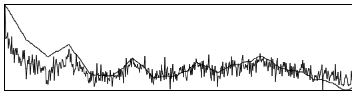
\includegraphics[clip,width=1.1\hsize]{img/POF.png}
  \caption{POF}\label{fig:POF}
\end{figure}

$$
\begin{aligned}
\mathrm{POF}[x_a, x_b]
&= \mathcal{F}^{-1}\left[\frac{\mathcal{F}\left[x_a(t)\right]^*}{|\mathcal{F}\left[x_a(t)\right]|}\mathcal{F}\left[x_b(t)\right]\right] \\
&= \mathcal{F}^{-1}\left[\frac{X_a^*(\omega)}{|X_a(\omega)|}X_b(\omega)\right]
\end{aligned}
$$


直接スペクトル拡散方式(図\ref{fig:DS})による測距システムの変復調方式を図\ref{fig:DME2}に示す.

\begin{figure}[p]\centering
  \hspace{-2mm}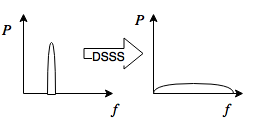
\includegraphics[clip,width=1.1\hsize]{img/DS.png}
  \caption{DS}\label{fig:DS}
\end{figure}

\begin{figure}[p]\centering
  \hspace{-2mm}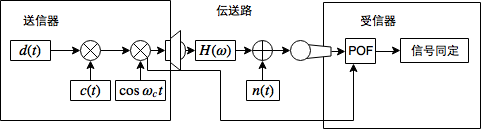
\includegraphics[clip,width=1.1\hsize]{img/DME2.png}
  \caption{DME2}\label{fig:DME2}
\end{figure}

\begin{figure}[p]\centering
  \hspace{-2mm}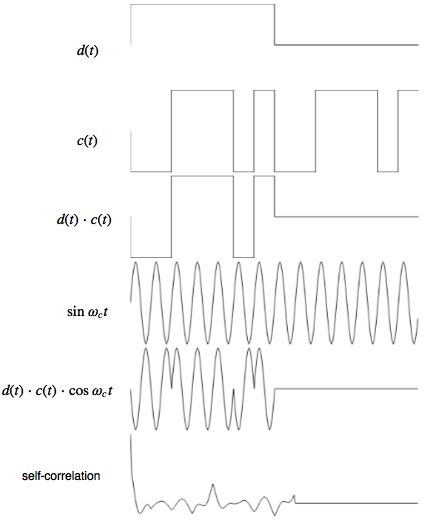
\includegraphics[clip,width=1.1\hsize]{img/DSSS.png}
  \caption{DSSS}\label{fig:DSSS}
\end{figure}

搬送波には1000Hzサイン波を,拡散符号にはM系列を用い,変調にはバイナリ位相シフトキーイング(BPSK)を使った.

復調した受信信号が雑音か有効な信号かを決定する処理を信号同定という.
伝送路における伝達関数 $H(\omega)$ において室内残響の影響
としてマルチパスによるを受けてしまう(図\ref{fig:multipath}).

\begin{figure}[pb]\centering
  \hspace{-2mm}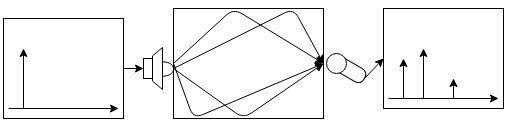
\includegraphics[clip,width=1.1\hsize]{img/multipath.png}
  \caption{multipath}\label{fig:multipath}
\end{figure}


そこで,同期パルスを測距用信号と,伝搬路を測定する参照波としてのサウンダ(sounder)信号の二つに分離した.
同期パルスから $n$ 秒後にサウンダ信号を送り,
その二つの信号の相関を取ることで,
背景雑音とは別にパルス位置を特定することが可能になる(図\ref{fig:sounder}).

\begin{figure}[pb]\centering
  \hspace{-2mm}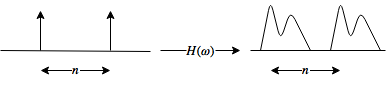
\includegraphics[clip,width=1.1\hsize]{img/sounder.png}
  \caption{sounder}\label{fig:sounder}
\end{figure}

さらにサウンダ信号と測距信号は互いに異なる同周期のM系列を用いた.
サウンダ信号と測距信号を判別しやすくするためである.

この時刻が $n$ 秒ずれた二つの信号に対して時間窓で区切って相互相関をとることで,
信号が最も相関している区間,つまり信号の位置を特定することができる.
最後に,その区間相関値を閾値処理することで信号の到来を決定する.
今回は最大相関値前方での40\%の相関値を超えたピークを到来時刻としている.

相関関数の計算にはウィーナー=ヒンチンの定理を使い周波数領域での複素乗算としてFFTを使って計算することで計算量を減らすことができる.
長さの異なる信号の高速フーリエ変換には重畳加算法\cite{overwrap}を使った.


\begin{figure}[p]
  \centering
  \includegraphics[clip,width=1.05\hsize]{img/026.jpeg}
  \caption{変復調回路}\label{fig:henpuku}
\end{figure}


\begin{figure}[p]
  \centering
  \includegraphics[clip,width=1.05\hsize]{img/029.jpeg}
  \caption{信号同定過程}\label{fig:shousai}
\end{figure}




\clearpage

\subsection{Barker coded chirpを用いたパルス圧縮}

これまでに測距・同期パルス(信号)の送受信による同期と測距および相対位置推定の手法について述べた.
ここでは,測距・同期精度を高くするための,信号検出手法について述べる.

信号検出においてSN比を最大化するフィルタを整合フィルタと呼び(図\ref{fig:matched_filter}),それは元信号との自己相関に等しい\cite{seigoufilter}.
理想的には整合フィルタを通した結果がデュラックのデルタ関数に近いことが望ましい.
しかしながら,そのような信号は短時間に大電力のパルスとなるため,送信機器の送信電力や回路の容量に物理的な制約があるため,そのような信号の送信は不可能である.
そこで,パルス圧縮と呼ばれる手法が使われている\cite{pulsecompress}.
パルス圧縮は,送信パルスを時間周波数方向へエネルギーを拡散させ,受信時にフィルタと高SN比で鋭いピークをもつようにする手法である.

音声パルスで同期する場合,音声信号のサンプリング周波数44100[Hz]と仮定すると,1サンプルあたりの時間解像度は約22.6$\mu$s,距離解像度は7.7mm(音速340[m/s]を仮定)となる.
人間の聴覚特性として$\pm$1msの誤差で別音源として聴こえることが知られている.
戦術の先行音効果により,必要な同期精度を$\pm$1msとすると,同期はおよそ$\pm$5サンプル以内の誤差に留める必要がある.
このような高精度のパルス検出のため,提案手法では複数のパルス圧縮方式を組み合わせる.

ここで,本手法に適用したパルス信号であるChirp信号について述べる.波形を図\ref{fig:chirpsig}に示し,スぺクトログラムを図\ref{fig:chirpsig2}に示す.
Chirp信号は,方形パルスを周波数方向へ掃引することで,図\ref{fig:chirppulse_amb}に示すように,通常パルスと同じ電力で時間方向の精度をより向上させることができることで知られている.
Barker符号(図\ref{fig:barkercode})はパルス圧縮の一種で,同期点以外での自己相関関数の絶対値の最大が$1/N$となる長さ$N$の有限長系列で,長さ13まで存在し,相関特性が長さ13の場合,ピークが13倍,レンジサイドローブが1/13倍となるような,ディラックの$\delta$関数に近い理想的な相関特性を持つことで知られている.

さらに,先行研究\cite{shibata13}のパルス圧縮に比べ,より強力なパルス圧縮として,
より狭い時間範囲にエネルギーを集中させることで,
上記の二つのパルス圧縮技術を組み合わせて,Chirp信号をBarker符号を用いてBPSKで変調した.
BPSKは位相0を0,位相$\pi$を1とする位相偏移変調で,位相変化を2値とする.
図\ref{fig:chirpqi}にBPSKの信号空間ダイアグラムを示す.

他にも,スマートデバイスのマイクロホンの周波数受信特性はそのハードウェアによって異なっている.
このため,BPSKの搬送波に特定の周波数を用いるのはハードウェアによっては最適ではない可能性がある.
これに対して,BPSKの搬送波に全帯域に対して掃引するChirp信号を用いる.
これにより,スマートデバイスのマイクロホンの周波数受信特性による差異を抑えることができると期待される.

\begin{figure}[pb]\centering
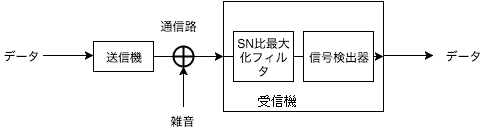
\includegraphics[clip,width=1.05\hsize]{img/matched_filter.png}
\caption{送受信モデルと整合フィルタ}\label{fig:matched_filter}

\end{figure}



\begin{figure}[pb]\centering
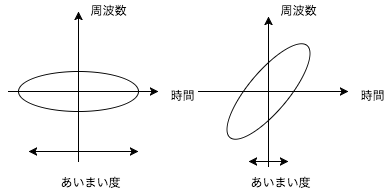
\includegraphics[clip,width=0.9\hsize]{img/aimai.png}\\
通常パルス~ ~ ~ ~ ~ ~ ~ ~ ~ ~ ~ Chirpパルス
\caption{Chirpパルスによるピーク曖昧度}\label{fig:chirppulse_amb}

\end{figure}

\begin{figure}[pb]\centering
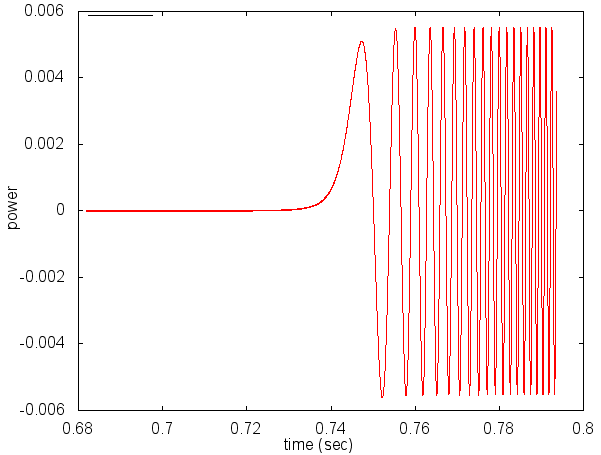
\includegraphics[clip,width=1.0\hsize]{img/chirp.png}
\caption{本手法で用いたChirp信号波形}\label{fig:chirpsig}

\end{figure}

\begin{figure}[pb]\centering
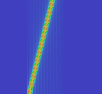
\includegraphics[clip,width=0.7\hsize]{img/chirp_spectogram.png}\\
\caption{本手法で用いたChirp信号スぺクトログラム}\label{fig:chirpsig2}

\end{figure}


\begin{figure}[pb]\centering
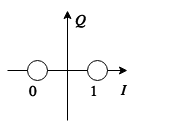
\includegraphics[clip,width=0.27\hsize]{img/chirp_qi.png}
\caption{BPSK信号空間ダイヤグラム}\label{fig:chirpqi}
\end{figure}




\begin{figure}[pb]\centering
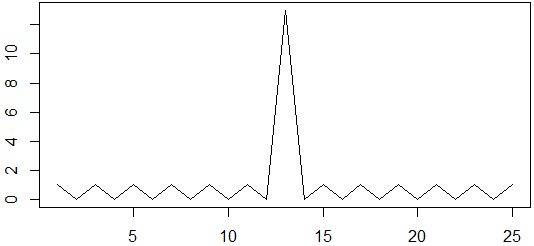
\includegraphics[clip,width=0.9\hsize]{img/barkercode.png}
\caption{Barker符号(13列)の自己相関形}\label{fig:barkercode}
\end{figure}

\begin{figure}[pb]\centering
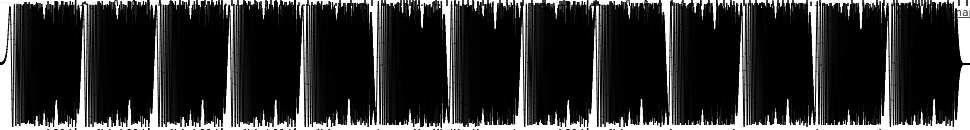
\includegraphics[clip,width=1.0\hsize]{img/barker_chirp.png}
\caption{13列Barker符号のBPSK変調信号(Chirp信号搬送波)}\label{fig:barker_chirp}
\end{figure}

\begin{figure}[pb]\centering
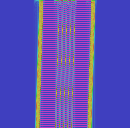
\includegraphics[clip,width=0.75\hsize]{img/barker_coded_chirp.png}
\caption{13列Barker符号のBPSK変調信号(Chirp信号搬送波)のスペクトルグラム(シミュレーション)}\label{fig:barker_coded_chirp}
\end{figure}


\begin{figure}[pb]\centering
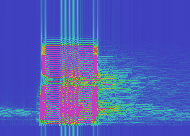
\includegraphics[clip,width=0.75\hsize]{img/barker_coded_chirp_err.png}
\caption{13列Barker符号のBPSK変調信号(Chirp信号搬送波)のスペクトルグラム
(MacBookAirによる実環境での自身の信号の計測結果)}\label{fig:barker_coded_chirp_err}
\end{figure}


\begin{figure*}[pb]\centering
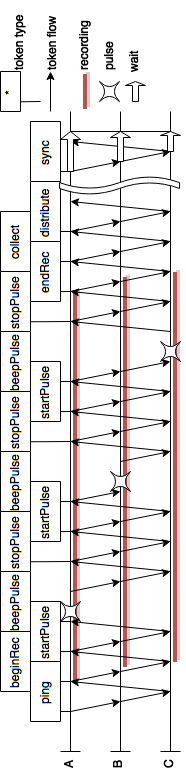
\includegraphics[clip,width=0.85\hsize]{img/flowchart.png}
\caption{システム動作のダイアグラム}\label{fig:pulsediagram}
\end{figure*}

\begin{figure}[pb]\centering
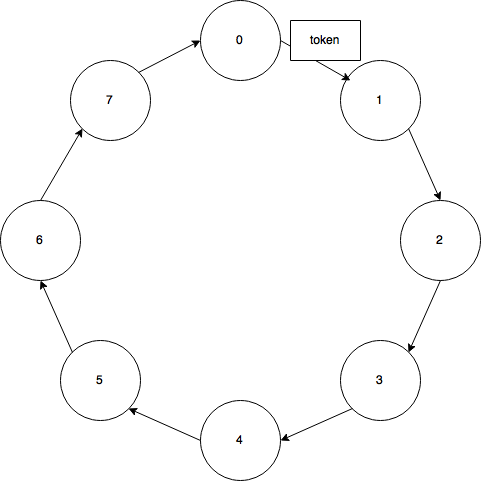
\includegraphics[clip,width=0.85\hsize]{img/chord_ring_network.png}
\caption{ネットワーク上でのトークンパッシング}\label{fig:scheduling}
\end{figure}


\begin{figure}[pb]\centering
\vspace{2mm}
\begin{small}
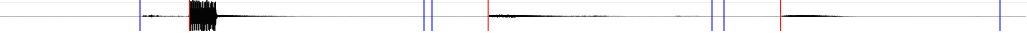
\includegraphics[clip,width=1.0\hsize]{img/rawdata.png}\\
A端末自身のパルス~ ~ ~ ~
B端末のパルス~ ~ ~ ~ ~
C端末のパルス\\\vspace{0.5mm}
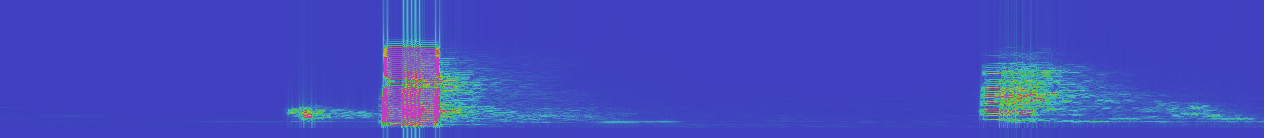
\includegraphics[clip,width=0.8\hsize]{img/spectrogram.png}\hspace{1cm}\\
A端末自身のパルス~ ~ ~ ~ ~ ~ ~ ~ ~
B端末のパルス\\\vspace{0.5mm}
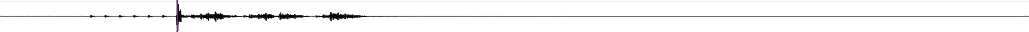
\includegraphics[clip,width=1.0\hsize]{img/corrA.png}\\
A端末のパルスに整合フィルタをかけたもの\\\vspace{0.5mm}
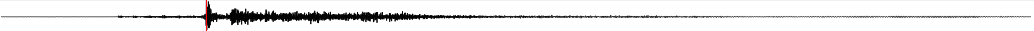
\includegraphics[clip,width=1.0\hsize]{img/corrB.png}\\
B端末のパルスに整合フィルタをかけたもの\\\vspace{0.5mm}
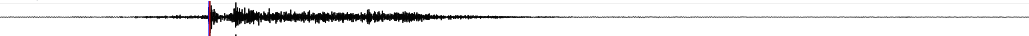
\includegraphics[clip,width=1.0\hsize]{img/corrC.png}\\
C端末のパルスに整合フィルタをかけたもの\\
\vspace{1mm}
\caption{A端末で観測したABC端末のパルス信号}\label{fig:corr}

\end{small}
\vspace{1mm}
\end{figure}
